\section{Results – Strategy S2: Iterative Single-Field}
\label{sec:eval-s2}

The \textbf{S2: Iterative Single-Field} strategy fills the template sequentially, invoking the LLM once per slot.
We evaluate three S2 variants:
\textbf{S2.0} = no few-shot examples on the original MUC-4 dataset;
\textbf{S2.1} = with few-shot examples on the original dataset;
\textbf{S2.2} = with few-shot examples on a modified dataset that mimics speech-style transcripts.

\subsection*{Headline Results}

\begin{figure}[h]
\centering
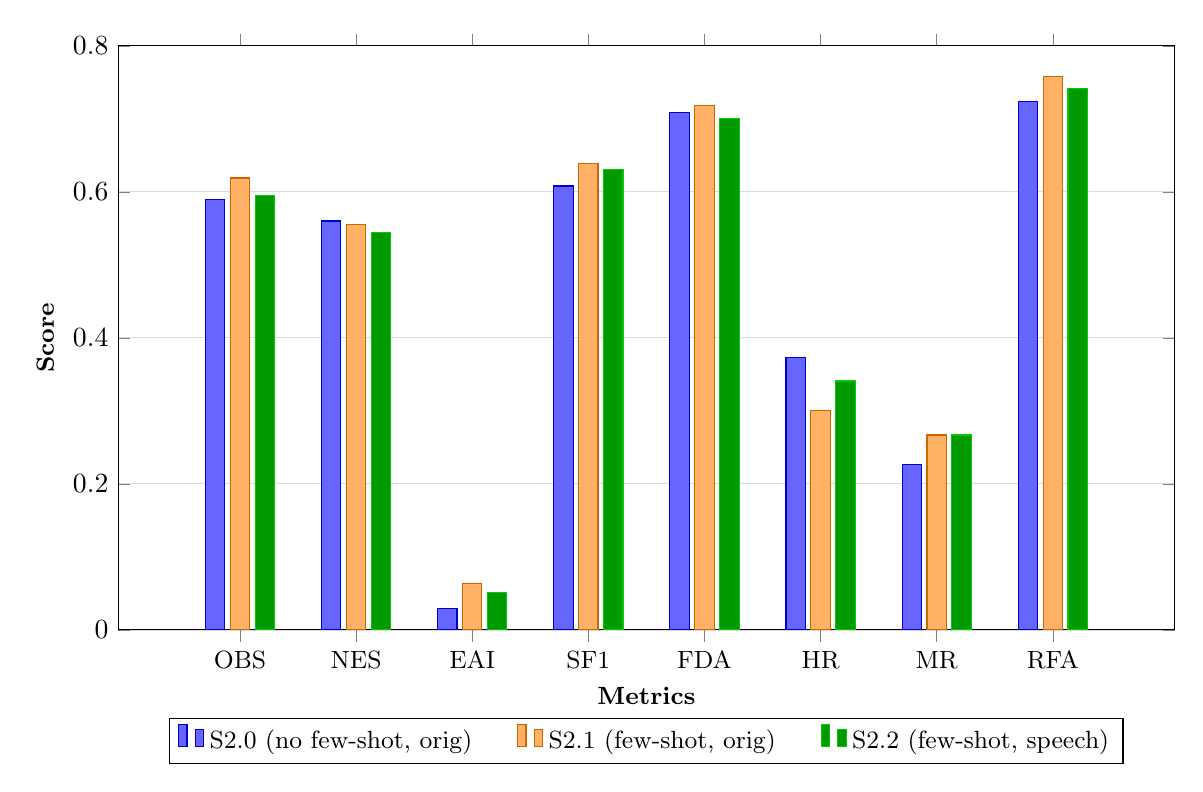
\begin{tikzpicture}
  \begin{axis}[
    width=15cm,
    height=9cm,
    ybar,
    bar width=7pt,
    ylabel={Score},
    ylabel style={font=\small\bfseries},
    xlabel={Metrics},
    xlabel style={font=\small\bfseries},
    symbolic x coords={OBS, NES, EAI, SF1, FDA, HR, MR, RFA},
    xtick=data,
    xticklabel style={font=\small},
    ymin=0,
    ymax=0.8,
    ytick={0, 0.2, 0.4, 0.6, 0.8},
    ymajorgrids=true,
    grid style={line width=0.3pt, draw=gray!30},
    legend style={
      at={(0.5,-0.15)},
      anchor=north,
      legend columns=3,
      font=\small,
      /tikz/every even column/.append style={column sep=0.5cm}
    },
    enlarge x limits=0.15,
  ]
  
  % S2.0 (no few-shot, orig) - Blue
  \addplot[fill=blue!60, draw=blue!80!black] coordinates {
    (OBS, 0.590)
    (NES, 0.560)
    (EAI, 0.029)
    (SF1, 0.608)
    (FDA, 0.709)
    (HR, 0.373)
    (MR, 0.226)
    (RFA, 0.724)
  };
  \addlegendentry{S2.0 (no few-shot, orig)}
  
  % S2.1 (few-shot, orig) - Orange
  \addplot[fill=orange!60, draw=orange!80!black] coordinates {
    (OBS, 0.619)
    (NES, 0.555)
    (EAI, 0.064)
    (SF1, 0.639)
    (FDA, 0.718)
    (HR, 0.301)
    (MR, 0.267)
    (RFA, 0.758)
  };
  \addlegendentry{S2.1 (few-shot, orig)}
  
  % S2.2 (few-shot, speech) - Green
  \addplot[fill=green!60!black, draw=green!80!black] coordinates {
    (OBS, 0.595)
    (NES, 0.544)
    (EAI, 0.051)
    (SF1, 0.631)
    (FDA, 0.700)
    (HR, 0.341)
    (MR, 0.267)
    (RFA, 0.742)
  };
  \addlegendentry{S2.2 (few-shot, speech)}
  
  \end{axis}
\end{tikzpicture}
\caption{Headline metrics for S2 variants on MUC-4 ($N{=}100$).}
\label{fig:s2-variants-bar}
\end{figure}

\paragraph{Per-field (reference for S2.1).}
\texttt{perpetratorOrganization} and \texttt{weapon} are strongest; \texttt{perpetratorIndividual} remains difficult; \texttt{incidentLocation} benefits from per-slot prompting.

\begin{table}[H]
    \centering
    \caption{Per-field average scores for S2.1 ($N{=}100$).}
    \label{tab:s2-perfield}
    \begin{tabular}{lcc}
        \toprule
        Field & Avg.\ Score & \#Docs \\
        \midrule
        incidentType & 0.520 & 100 \\
        incidentDate & 0.550 & 100 \\
        incidentLocation & 0.597 & 100 \\
        incidentStage & 0.700 & 100 \\
        perpetratorIndividual & 0.564 & 100 \\
        perpetratorOrganization & 0.738 & 100 \\
        target & 0.608 & 100 \\
        victim & 0.543 & 100 \\
        weapon & 0.751 & 100 \\
        \midrule
        \textbf{Overall (OBS)} & \textbf{0.619} & \textbf{900 comps} \\
        \bottomrule
    \end{tabular}
\end{table}

\subsection*{Latency}

\begin{figure}[H]
\centering
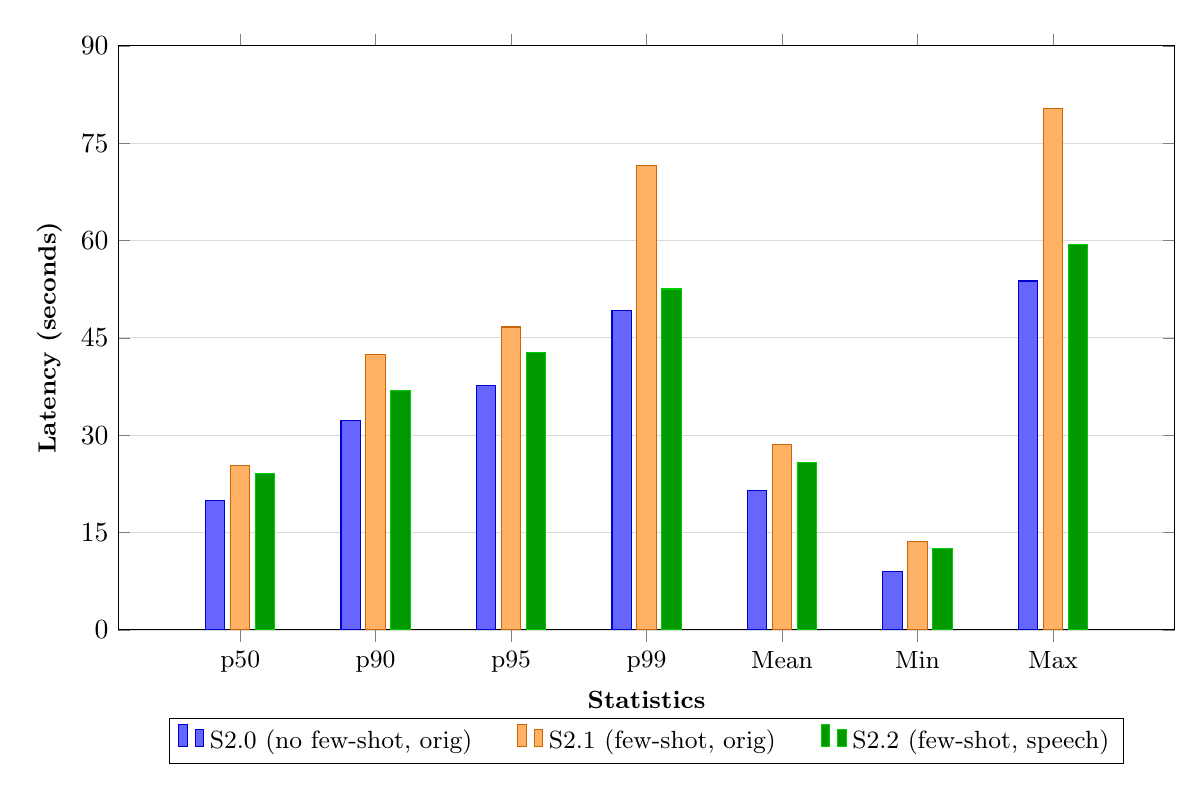
\begin{tikzpicture}
  \begin{axis}[
    width=15cm,
    height=9cm,
    ybar,
    bar width=7pt,
    ylabel={Latency (seconds)},
    ylabel style={font=\small\bfseries},
    xlabel={Statistics},
    xlabel style={font=\small\bfseries},
    symbolic x coords={p50, p90, p95, p99, Mean, Min, Max},
    xtick=data,
    xticklabel style={font=\small},
    ymin=0,
    ymax=90,
    ytick={0, 15, 30, 45, 60, 75, 90},
    ymajorgrids=true,
    grid style={line width=0.3pt, draw=gray!30},
    legend style={
      at={(0.5,-0.15)},
      anchor=north,
      legend columns=3,
      font=\small,
      /tikz/every even column/.append style={column sep=0.5cm}
    },
    enlarge x limits=0.15,
  ]
  
  % S2.0 (no few-shot, orig) - Blue
  \addplot[fill=blue!60, draw=blue!80!black] coordinates {
    (p50, 19.97)
    (p90, 32.24)
    (p95, 37.69)
    (p99, 49.26)
    (Mean, 21.48)
    (Min, 9.01)
    (Max, 53.76)
  };
  \addlegendentry{S2.0 (no few-shot, orig)}
  
  % S2.1 (few-shot, orig) - Orange
  \addplot[fill=orange!60, draw=orange!80!black] coordinates {
    (p50, 25.35)
    (p90, 42.48)
    (p95, 46.68)
    (p99, 71.52)
    (Mean, 28.58)
    (Min, 13.60)
    (Max, 80.28)
  };
  \addlegendentry{S2.1 (few-shot, orig)}
  
  % S2.2 (few-shot, speech) - Green
  \addplot[fill=green!60!black, draw=green!80!black] coordinates {
    (p50, 24.07)
    (p90, 36.93)
    (p95, 42.81)
    (p99, 52.53)
    (Mean, 25.83)
    (Min, 12.51)
    (Max, 59.36)
  };
  \addlegendentry{S2.2 (few-shot, speech)}
  
  \end{axis}
\end{tikzpicture}
\caption{Latency statistics for S2 variants (seconds).}
\label{fig:s2-latency-bar}
\end{figure}


\subsection*{Cost Analysis (S2: Single-Field Iterative)}

\textbf{Assumptions.} We extract each of the $F{=}9$ MUC-4 slots with a separate \textit{GPT-5} call. 
Per field (average): $i_f{=}1{,}500$ input tokens, $o_f{=}50$ output tokens. 
Verification with \textit{GPT-5-mini} is done \emph{once per record} (not per field) with $V_{\text{in}}{=}1{,}000$, $V_{\text{out}}{=}100$. 
If audio is used, add Whisper transcription for $D$ minutes (once per record).

\textbf{Prices.} GPT-5: input \$1.25/M, output \$10.00/M. GPT-5-mini: input \$0.25/M, output \$2.00/M. Whisper: \$0.006/min.

\textbf{Formula.}
\[
\text{Cost}_{\text{S2}} =
\underbrace{
\sum_{f=1}^{F}\!\left(\frac{i_f}{10^6}p_{\text{in}}+\frac{o_f}{10^6}p_{\text{out}}\right)
}_{\text{per-field extraction on GPT-5}}
+
\underbrace{
\frac{V_{\text{in}}}{10^6}p^{(\text{mini})}_{\text{in}}+\frac{V_{\text{out}}}{10^6}p^{(\text{mini})}_{\text{out}}
}_{\text{single verification on GPT-5-mini}}
+0.006\cdot D
\]

\textbf{Per-record (no audio).}
\[
9\times\Big(
\underbrace{\tfrac{1500}{10^6}\!\cdot\!1.25}_{\$0.001875}
+\underbrace{\tfrac{50}{10^6}\!\cdot\!10.00}_{\$0.000500}
\Big)
+\underbrace{\tfrac{1000}{10^6}\!\cdot\!0.25}_{\$0.000250}
+\underbrace{\tfrac{100}{10^6}\!\cdot\!2.00}_{\$0.000200}
=\mathbf{\$0.02183}\ (\approx 2.18\text{¢/doc})
\]

\textbf{With audio (Whisper).} Add $0.006\cdot D$. For $D{=}1$ min: $\$0.02183+0.006=\mathbf{\$0.02783}$ (\(\approx 2.78\,\text{¢}\)).

\textbf{Takeaway.} With these settings, S2 costs \(\approx 3.03\times\) S1 (\$0.02183 vs.\ \$0.00720 per doc, no audio), driven by the $F$ separate extraction calls; verification once per record keeps the verifier overhead small.



\subsection*{Insights}

\begin{itemize}
    \item \textbf{Few-shot improves accuracy and calibrates fills.} S2.1 vs.\ S2.0: OBS +0.029, SF1 +0.031; hallucinations drop substantially (HR 0.373$\rightarrow$0.301) with a small FDA gain (0.709$\rightarrow$0.718). Misses rise (MR 0.226$\rightarrow$0.267), indicating a shift toward more conservative fills.
    \item \textbf{Iterative prompting helps location.} S2.1 attains \texttt{incidentLocation} 0.597 (baseline regime), noticeably higher than S1’s single-pass numbers, consistent with field-focused instructions improving locality grounding.
    \item \textbf{Speech-style robustness with mild cost.} S2.2 maintains competitive OBS/SF1 (0.595/0.631) and similar MR to S2.1, but with lower FDA (0.700) and higher HR (0.341). RFA remains strong (0.742), suggesting good quality when both sides produce values, but overall more cautious/variable fill decisions on spoken-like inputs.
    \item \textbf{Persistent hard spot: \texttt{perpetratorIndividual}.} Scores remain low across variants due to sparse gold and ambiguous mentions; even with per-slot focus, recall lags compared to \texttt{weapon} and \texttt{perpetratorOrganization}.
    \item \textbf{Latency–quality profile.} All S2 variants are faster than the best S1 accuracy setting (S1.1). S2.0 is the speed leader (p50 $\sim$20\,s/doc) but has higher HR; S2.1 delivers the best accuracy at a moderate latency increase; S2.2 offers a middle ground for speech-like text with shorter tails than S1.1.
\end{itemize}
